\tikzset{
pattern size/.store in=\mcSize,
pattern size = 5pt,
pattern thickness/.store in=\mcThickness,
pattern thickness = 0.3pt,
pattern radius/.store in=\mcRadius,
pattern radius = 1pt}
\makeatletter
\pgfutil@ifundefined{pgf@pattern@name@_iy1rqtf17}{
\pgfdeclarepatternformonly[\mcThickness,\mcSize]{_iy1rqtf17}
{\pgfqpoint{0pt}{0pt}}
{\pgfpoint{\mcSize+\mcThickness}{\mcSize+\mcThickness}}
{\pgfpoint{\mcSize}{\mcSize}}
{
\pgfsetcolor{\tikz@pattern@color}
\pgfsetlinewidth{\mcThickness}
\pgfpathmoveto{\pgfqpoint{0pt}{0pt}}
\pgfpathlineto{\pgfpoint{\mcSize+\mcThickness}{\mcSize+\mcThickness}}
\pgfusepath{stroke}
}}
\makeatother
\tikzset{every picture/.style={line width=0.75pt}} %set default line width to 0.75pt

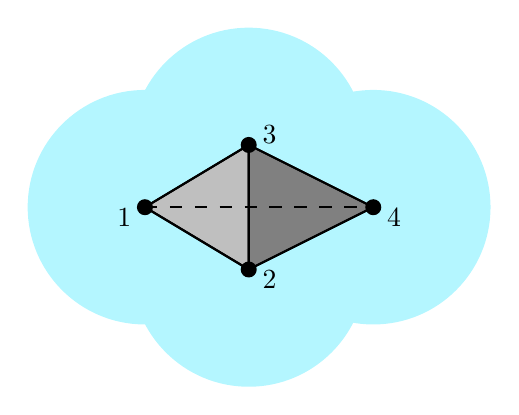
\begin{tikzpicture}[x=0.75pt,y=0.75pt,yscale=-1,xscale=1]

% COORDINATES

\coordinate (1) at (10,30);
\coordinate (3) at (60,0);
\coordinate (2) at (60,60);
\coordinate (4) at (120,30);

\def\points{
    (1),
    (2),
    (3),
    (4)
}

\def\radius{56}

% BALLS

\foreach \p in \points{
    \draw [color={rgb, 255:red, 180; green, 246; blue, 255 }]
          [fill ={rgb, 255:red, 180; green, 246; blue, 255 }]
            \p circle[radius=\radius];
}

% TRIANGLE

\draw [black, fill=lightgray] (1) -- (2) -- (3) -- cycle ;
\draw [black, fill=gray] (2) -- (3) -- (4) -- cycle ;

% VERTICES

\foreach \p [count=\pi] in \points{
    \draw [black, fill=black]\p circle[radius=3.35];
}

% EDGES

\draw (1)--(2) ;
\draw (1)--(3) ;
\draw [dash pattern={on 4.5pt off 4.5pt}] (1)--(4) ;
\draw (2)--(3) ;
\draw (2)--(4) ;
\draw (3)--(4) ;

% LABELS

\draw {(1)}+(-10,5) node {1};
\draw {(2)}+(10,5) node {2};
\draw {(3)}+(10,-5) node {3};
\draw {(4)}+(10,5) node {4};

\end{tikzpicture}
